\documentclass{standalone}

%----------------------------------------------------------------------------------------------%
%                                 Packages and basic declarations
%----------------------------------------------------------------------------------------------%

\usepackage{amsmath}
\usepackage{mathrsfs}
\usepackage{pgf}
\usepackage{tikz}
\usepackage{verbatim}


\usetikzlibrary{arrows}



%----------------------------------------------------------------------------------------------%
%----------------------------------------------------------------------------------------------%
%                                            DOCUMENT STARTS
%----------------------------------------------------------------------------------------------%
%----------------------------------------------------------------------------------------------%


\begin{document}

%----------------------------------------------------------------------------------------------%
%                Single RVE with applied constant strain, only debonded
%----------------------------------------------------------------------------------------------%
 
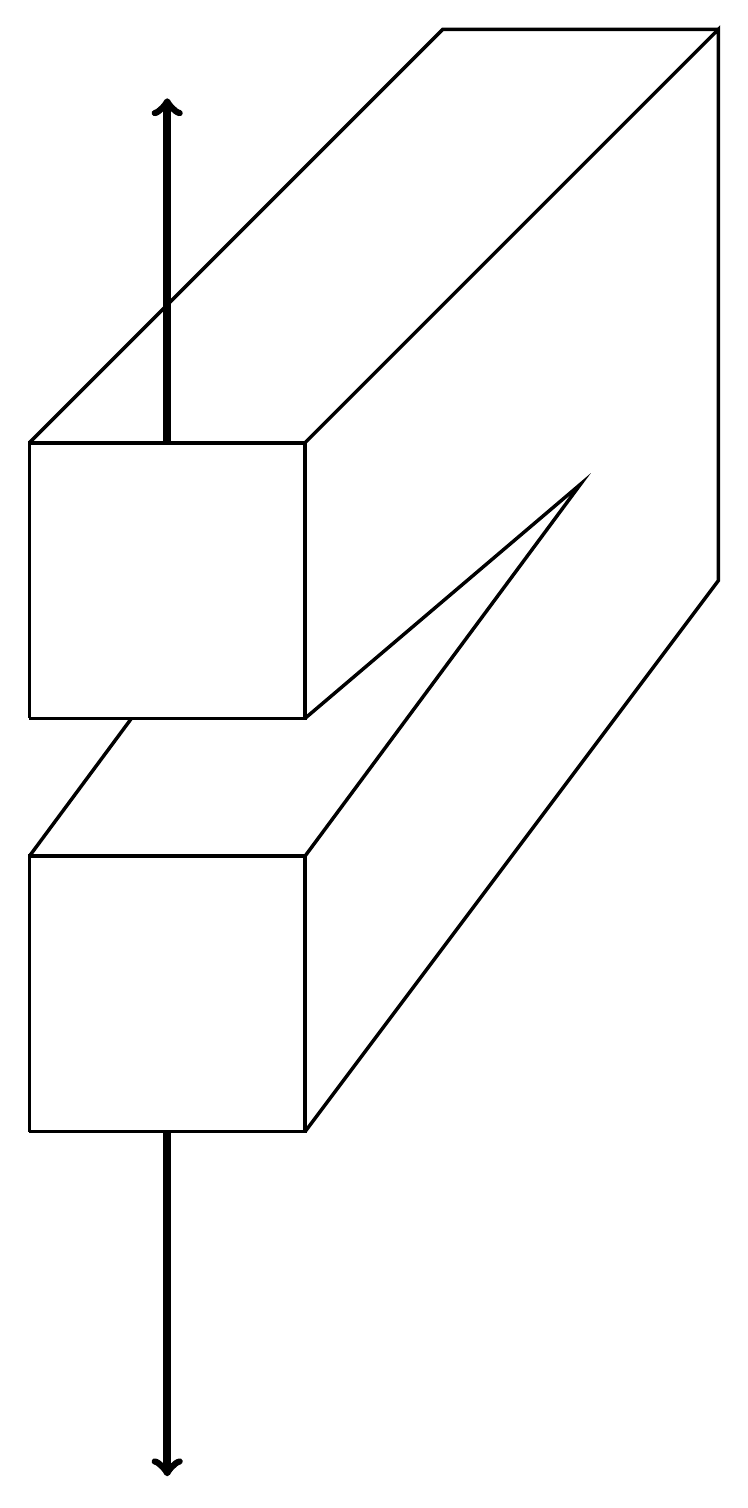
\begin{tikzpicture}[x=3.5cm, y=3.5cm]
\def\linewidth{1.25pt}


\draw[black,line width=\linewidth] (0,0)--(1,0)--(1,1)--(0,1)--(0,0);

\draw[black,line width=\linewidth] (1,1)--(2,2.35)--(1,1.5);

\draw[black,line width=\linewidth] (1,0)--(2.5,2)--(2.5,4)--(1,2.5);

\draw[black,line width=\linewidth] (2.5,4)--(1.5,4)--(0,2.5);

\draw[black,line width=\linewidth] (0,1)--(1,2.35);

\filldraw[white] (0,1.5)--(1,1.5)--(1,2.5)--(0,2.5)--(0,1.5);

\draw[black,line width=\linewidth] (0,1.5)--(1,1.5)--(1,2.5)--(0,2.5)--(0,1.5);

\draw[black,->,line width=2.25*\linewidth] (0.5,2.5) -- (0.5,3.75);

\draw[black,->,line width=2.25*\linewidth] (0.5,0) -- (0.5,-1.25);

\end{tikzpicture}

\end{document}